\documentclass[tikz, border=10pt]{standalone}
\usepackage{pgfplots}
\usepackage{amsmath}
\usetikzlibrary{backgrounds}
\pgfplotsset{compat=1.18}

\begin{document}
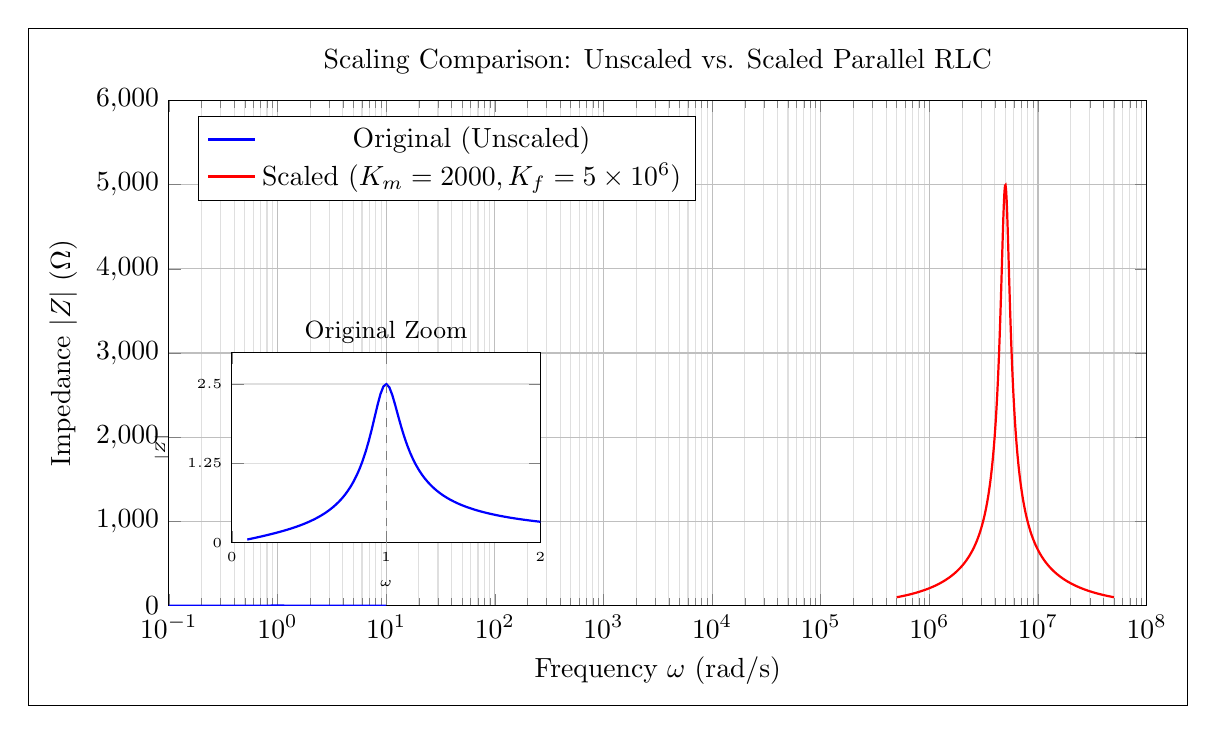
\begin{tikzpicture}[show background rectangle]
    \begin{semilogxaxis}[
        width=14cm, height=8cm,
        name=mainplot,
        title={Scaling Comparison: Unscaled vs. Scaled Parallel RLC},
        xlabel={Frequency $\omega$ (rad/s)},
        ylabel={Impedance $|Z|$ ($\Omega$)},
        grid=both,
        xmin=0.1, xmax=10^8,
        ymin=0, ymax=6000,
        minor grid style={gray!25},
        major grid style={gray!50},
        legend pos=north west,
    ]

    % Unscaled: R=2.5, L=0.5, C=2
    \addplot[blue, thick, domain=0.1:10, samples=200] { 1 / sqrt( (1/2.5)^2 + (2*x - 2/x)^2 ) };
    \addlegendentry{Original (Unscaled)}

    % Scaled: R'=5000, L'=0.2mH, C'=0.2nF
    % Km=2000, Kf=5e6. Scaling [0.1:10] by 5e6 gives [5e5:5e7]
    \addplot[red, thick, domain=5e5:5e7, samples=400] { 5000 / sqrt( 1 + 25 * (x/5e6 - 5e6/x)^2 ) };
    \addlegendentry{Scaled ($K_m=2000, K_f=5 \times 10^6$)}

    \end{semilogxaxis}

    % Inset Zoom for Unscaled Response
    \begin{axis}[
        at={(mainplot.south west)},
        xshift=0.8cm,
        yshift=0.8cm,
        width=5.5cm, height=4cm,
        anchor=south west,
        title={Original Zoom},
        title style={font=\small, yshift=-1.5ex},
        xlabel={$\omega$},
        ylabel={$|Z|$},
        tick label style={font=\tiny},
        label style={font=\tiny},
        grid=both,
        xmin=0, xmax=2,
        ymin=0, ymax=3,
        xtick={0, 1, 2},
        ytick={0, 1.25, 2.5},
        minor grid style={gray!10},
        major grid style={gray!25},
        axis background/.style={fill=white},
    ]
        \addplot[blue, thick, domain=0.1:2, samples=100] { 1 / sqrt( (1/2.5)^2 + (2*x - 2/x)^2 ) };
        \draw[dashed, gray] (axis cs:1, 0) -- (axis cs:1, 2.5);
    \end{axis}
\end{tikzpicture}
\end{document}
